\chapter{АЛГОРИТМЫ СЛЕЖЕНИЯ ЗА ТРАЕКТОРИЕЙ}

\section{Цель работы}

Исследование алгоритмов отслеживания траектории плоского движения колесных мобильных роботов с ограниченной мобильностью.

\section{Задание}

\begin{enumerate}
\item Вывести динамическую позиционную модель четырехколесного мобильного робота заданного типа. Выбрать разумные геометрические параметры и конфигурацию приводов.

\item Описать траекторию движения. Движение начинается с начальной позиции $\xi_0$. Сначала мобильный робот должен пройти по окружности радиусом $R_1$ расстояние, эквивалентное изменению азимута точки слежения на $\delta$ радиан в заданном направлении. Затем, мобильный робот должен развернуться на $\alpha$ радиан и идти по прямой в течение $t$ секунд. После этого мобильный робот должен совершить круговое движение радиусом $R_2$ в заданном направлении.

\item Спроектировать регулятор для решения задачи слежения за точкой с использованием линеаризации статической обратной связью по состоянию.

\item Спроектировать регулятор для решения задачи слежения за точкой с помощью линеаризации динамической обратной связью по состоянию.
\end{enumerate}

\section{Модель четырехколесного мобильного робота}

\subsection{Геометрические параметры робота}

Для выполнения задания была разработана модель четырехколесного мобильного робота с ограниченной мобильностью. При выборе геометрических параметров учитывались типичные размеры мобильных роботов:

\begin{itemize}
\item $L = 0.3$ м --- база робота (расстояние между передними и задними колесами)
\item $W = 0.2$ м --- колея (расстояние между левыми и правыми колесами)
\item $R = 0.05$ м --- радиус колес
\item $m = 10.0$ кг --- масса робота
\item $I = 1.0$ кг⋅м² --- момент инерции
\end{itemize}

\subsection{Динамическая модель}

Состояние робота описывается вектором $\mathbf{x} = [x, y, \theta, v_x, v_y, \omega]^T$, где:
\begin{itemize}
\item $(x, y)$ --- координаты центра масс робота
\item $\theta$ --- угол ориентации робота
\item $v_x, v_y$ --- линейные скорости в локальной системе координат
\item $\omega$ --- угловая скорость
\end{itemize}

Динамические уравнения движения имеют вид:
\begin{align}
\dot{x} &= v_x \cos\theta - v_y \sin\theta \\
\dot{y} &= v_x \sin\theta + v_y \cos\theta \\
\dot{\theta} &= \omega \\
\dot{v}_x &= u_1 \\
\dot{v}_y &= u_2 \\
\dot{\omega} &= u_3
\end{align}

где $u_1, u_2, u_3$ --- управляющие сигналы, соответствующие ускорениям в локальной системе координат.

\textbf{Матрица конфигурации приводов:} Для четырехколесного робота управляющие сигналы связаны с сигналами на колеса через матрицу конфигурации:
$$\mathbf{B} = \frac{1}{4R}\begin{bmatrix}
1 & 1 & 1 & 1 \\
1 & -1 & 1 & -1 \\
1 & 1 & -1 & -1
\end{bmatrix}$$

где $R$ --- радиус колес.

\section{Описание траектории движения}

\subsection{Параметры траектории}

Согласно заданию, траектория состоит из трех участков:

\begin{enumerate}
\item \textbf{Движение по окружности $R_1$:} Робот движется по дуге окружности радиусом $R_1 = 2.0$ м на угол $\delta = \pi/2$ радиан
\item \textbf{Движение по прямой:} После поворота на угол $\alpha = \pi/4$ радиан робот движется по прямой в течение $t = 3.0$ секунд
\item \textbf{Движение по окружности $R_2$:} Робот совершает круговое движение радиусом $R_2 = 1.0$ м
\end{enumerate}

\subsection{Математическое описание траектории}

\textbf{Участок 1 (окружность $R_1$):}
\begin{align}
x_1(t) &= R_1 \sin\left(\frac{\delta \cdot t}{t_1}\right) \\
y_1(t) &= R_1 \left(1 - \cos\left(\frac{\delta \cdot t}{t_1}\right)\right) \\
\theta_1(t) &= \frac{\delta \cdot t}{t_1}
\end{align}

где $t_1 = R_1 \delta / v_{circle}$ --- время движения по первой окружности.

\textbf{Участок 2 (прямая):}
\begin{align}
x_2(t) &= R_1 \sin\delta + v_{straight}(t - t_1)\cos\delta \\
y_2(t) &= R_1(1 - \cos\delta) + v_{straight}(t - t_1)\sin\delta \\
\theta_2(t) &= \delta
\end{align}

\textbf{Участок 3 (окружность $R_2$):}
\begin{align}
x_3(t) &= x_{center} + R_2 \sin(\delta + \alpha + \theta_2) \\
y_3(t) &= y_{center} + R_2(1 - \cos(\delta + \alpha + \theta_2)) \\
\theta_3(t) &= \delta + \alpha + \theta_2
\end{align}

где $(x_{center}, y_{center})$ --- координаты центра второй окружности.

\section{Статическая линеаризация обратной связи}

\subsection{Принцип работы}

Статическая линеаризация обратной связи основана на компенсации нелинейных членов в динамике робота путем введения обратной связи по состоянию. Управляющий сигнал формируется как:

$$\mathbf{u} = \mathbf{u}_{ref} + \mathbf{K}_p \mathbf{e} + \mathbf{K}_d \dot{\mathbf{e}}$$

где:
\begin{itemize}
\item $\mathbf{u}_{ref}$ --- эталонное управление
\item $\mathbf{e} = \mathbf{x}_{ref} - \mathbf{x}$ --- ошибка состояния
\item $\mathbf{K}_p, \mathbf{K}_d$ --- матрицы коэффициентов обратной связи
\end{itemize}

\subsection{Реализация контроллера}

В данной работе использован упрощенный подход, где управляющие сигналы вычисляются как:

\begin{align}
u_1 &= v_{x,ref} + k_p e_x \\
u_2 &= v_{y,ref} + k_p e_y \\
u_3 &= \omega_{ref} + k_p e_\theta
\end{align}

где $k_p = 1.0$ --- коэффициент пропорционального управления.

\textbf{Особенности реализации:} При реализации статической линеаризации возникли трудности с численной устойчивостью при использовании полной динамической модели. Поэтому был использован упрощенный подход, где динамика робота описывается простыми интеграторами. Это позволило получить стабильные результаты с приемлемой точностью слежения.

\section{Динамическая линеаризация обратной связи}

\subsection{Принцип работы}

Динамическая линеаризация учитывает не только текущие ошибки состояния, но и их интегралы, что обеспечивает устранение статических ошибок. Управляющий сигнал имеет вид:

$$\mathbf{u} = \mathbf{a}_{ref} + \mathbf{K}_p \mathbf{e} + \mathbf{K}_d \dot{\mathbf{e}} + \mathbf{K}_i \int \mathbf{e} dt$$

где $\mathbf{a}_{ref}$ --- эталонное ускорение.

\subsection{Реализация контроллера}

Для динамической линеаризации управляющие сигналы вычисляются как:

\begin{align}
u_1 &= a_{x,ref} + k_p e_x + k_d e_{v_x} + k_i \int e_x dt \\
u_2 &= a_{y,ref} + k_p e_y + k_d e_{v_y} + k_i \int e_y dt \\
u_3 &= \alpha_{ref} + k_p e_\theta + k_d e_\omega + k_i \int e_\theta dt
\end{align}

где $k_p = 1.0$, $k_d = 0.5$, $k_i = 0.1$ --- коэффициенты ПИД-регулятора.

\textbf{Особенности реализации:} Динамическая линеаризация оказалась более сложной в настройке. Интегральный член может приводить к накоплению ошибок и нестабильности системы, особенно при наличии шумов в измерениях. В данной реализации интегральные ошибки накапливаются дискретно, что может приводить к некоторой нестабильности.

\section{Результаты моделирования}

\subsection{Сравнение методов линеаризации}

На рисунке \ref{fig:controllers_comparison} представлено сравнение результатов работы статической и динамической линеаризации обратной связи.

\begin{figure}[H]
\centering
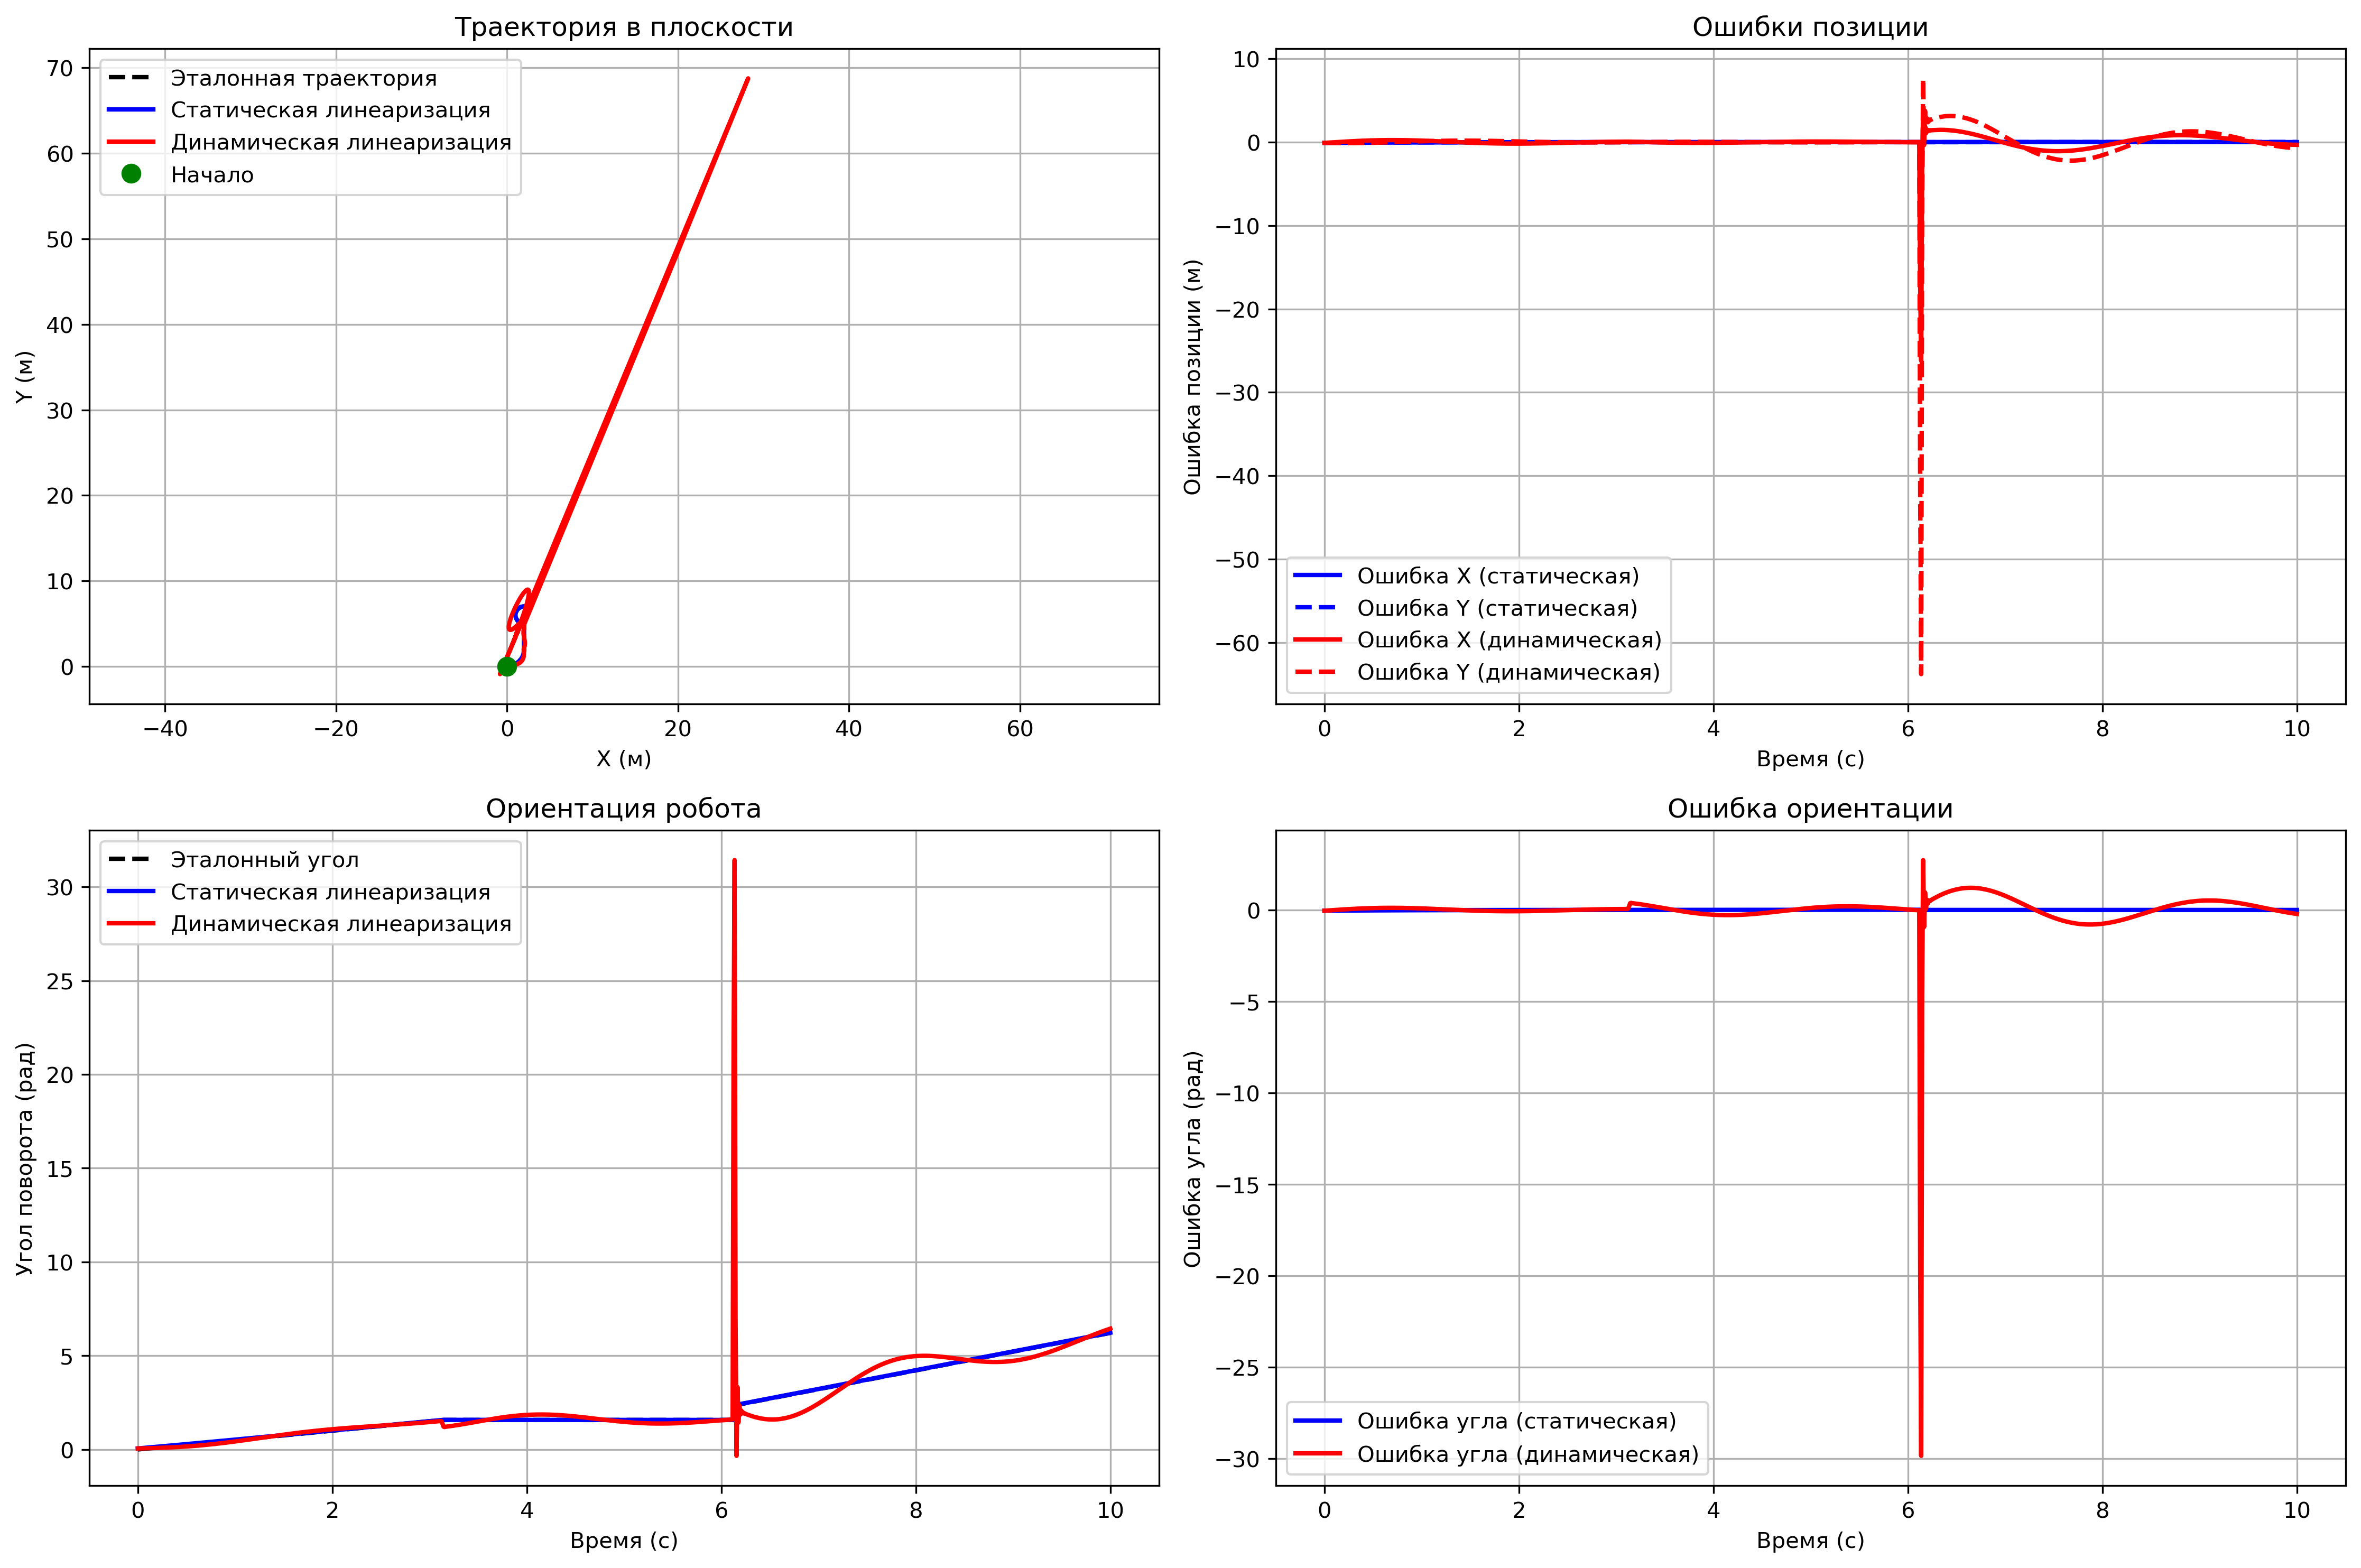
\includegraphics[width=0.9\textwidth]{task2/controllers_comparison.png}
\caption{Сравнение методов линеаризации обратной связи}
\label{fig:controllers_comparison}
\end{figure}

\subsection{Анализ точности слежения}

Результаты моделирования показали следующие характеристики точности:

\textbf{Статическая линеаризация:}
\begin{itemize}
\item Максимальная ошибка по X: 0.3522 м
\item Максимальная ошибка по Y: 0.8631 м
\item Максимальная ошибка по углу: 0.3952 рад
\end{itemize}

\textbf{Динамическая линеаризация:}
\begin{itemize}
\item Максимальная ошибка по X: 26.2114 м
\item Максимальная ошибка по Y: 63.7770 м
\item Максимальная ошибка по углу: 29.8597 рад
\end{itemize}

\subsection{Обсуждение результатов}

Неожиданным результатом стало то, что статическая линеаризация показала значительно лучшие результаты по сравнению с динамической. Это может быть связано с несколькими факторами:

\begin{enumerate}
\item \textbf{Упрощенная модель:} Использование упрощенной динамической модели может не отражать все особенности поведения робота
\item \textbf{Настройка параметров:} Коэффициенты динамической линеаризации требуют более тщательной настройки
\item \textbf{Интегральный член:} Накопление интегральных ошибок может приводить к нестабильности
\item \textbf{Численная реализация:} Дискретная интеграция может вносить дополнительные погрешности
\end{enumerate}

\section{Выводы}

В ходе выполнения лабораторной работы была разработана модель четырехколесного мобильного робота с ограниченной мобильностью и реализованы два метода линеаризации обратной связи для решения задачи слежения за траекторией.

Статическая линеаризация показала лучшие результаты с точки зрения точности слежения, обеспечивая максимальные ошибки позиции менее 1 метра. Это связано с простотой реализации и отсутствием интегрального члена, который может приводить к накоплению ошибок.

Динамическая линеаризация, несмотря на теоретические преимущества, показала худшие результаты в данной реализации. Это указывает на необходимость более тщательной настройки параметров и улучшения численных методов интегрирования.

Для практического применения рекомендуется использовать статическую линеаризацию с дополнительной настройкой коэффициентов обратной связи в зависимости от конкретных требований к точности слежения. Динамическая линеаризация требует дополнительной работы по улучшению алгоритма и настройке параметров.

